% Provenance (never printed): see sources/outline_sources.md (Year 2: the Himalaya and Tibet;
% the Andes; crustal thickening and plateaus). Himalayan units, thrusts and rates after Lave
% and Avouac (2000), Ader et al. (2012), Cattin et al. (2001), Dong et al. (2026, STDS);
% Asian extrusion after Jiao et al. (2023); Tibetan rifts after Wang et al. (2021); Central
% Andes after Gerbault et al. (2005); flat slabs after Gauthier et al. (2024). Relief from
% ETOPO1 (figdata/bachelor-2/plateaus.py); plate velocities from NNR-MORVEL56 (Book 2 ledger
% row nnr56:poles). Exercise and problem values in the Book 4 scratch calculator
% calc/ch14.py.
\chapter{碰撞造山带与安第斯型造山带比较}\label{ch:b2:himalaya-andes}

地球上有两座高原，绵延数百千米，海拔超过四千米。
西藏隆起于印度撞上亚洲之处，两块大陆在它们之间的大洋消失之后相遇。
阿尔蒂普拉诺高原隆起于大洋板块（纳斯卡板块）仍在南美洲之下俯冲之处，
此处并无大陆到来。两种不同的动力机制塑造了两种相似的地貌。
本章分别剖析这两条\omterm{def:b2:alpine-orogen:orogen}{造山带}，测量其\omterm{def:b2:himalaya-andes:thickening}{地壳增厚}的程度及原因，
并探讨是什么阻止它们继续抬升。
% ledger: lave00:setting, gerbault05:andes, data:b4-etopo-tibet, data:b4-etopo-andes

\begin{recall}
\textbf{来自高中分册}：大陆碰撞与缝合带；印度的
北向漂移、减速及碰撞年代的争议；青藏高原海拔
约 \qty{4600}{m}，地壳厚约 \qty{70}{km}。\textbf{来自本科一年级分册}：
艾里均衡与布格板片；活动大陆边缘、俯冲板片、火山弧与
弧沟间隙；由角速度求板块速度；拜尔利定律；矩
震级。\textbf{来自\cref{ch:b2:crustal-melting}}：喜马拉雅\omterm{def:b2:crustal-melting:leucogranite}{淡色花岗岩}。
\textbf{来自\cref{ch:b2:alpine-orogen}}：\omterm{def:b2:alpine-orogen:orogen}{造山带}、\omterm{def:b2:alpine-orogen:nappes}{推覆体}、\omterm{def:b2:alpine-orogen:decollement}{滑脱面}、薄皮与
\omterm{def:b2:alpine-orogen:skin}{厚皮构造}、\omterm{def:b2:alpine-orogen:ftb}{褶皱–冲断带}、\omterm{def:b2:alpine-orogen:foreland}{前陆盆地}、\omterm{def:b2:alpine-orogen:balanced}{平衡剖面}。
\end{recall}

\begin{definition}[碰撞造山带；安第斯型造山带]\label{def:b2:himalaya-andes:types}
称\emph{碰撞造山带}\index{碰撞造山带}为由两个大陆边缘
在其间大洋消亡后汇聚而成的\omterm{def:b2:alpine-orogen:orogen}{造山带}；其轴线为缝合带。
而\emph{安第斯型造山带}\index{安第斯型造山带}是建造在
大洋–\omterm{def:b2:alpine-orogen:obduction}{大陆俯冲}带的上盘板块之上、俯冲仍在其下进行的\omterm{def:b2:alpine-orogen:orogen}{造山带}；其轴线
为火山弧。
\end{definition}


\section{印度与亚洲}\label{sec:b2:himalaya-andes:himalaya}

约 5000 万年前，印度沿印度河–雅鲁藏布
缝合带与欧亚大陆南缘相遇（亦称印度河–雅鲁藏布缝合带）；确切年代仍有争议，如高中分册所示。
汇聚并未停止。今日印度与亚洲相互靠近，
速率约为每年 \qty{40}{mm}；由 NNR-MORVEL56 板块模型的角速度可知，
印度相对于欧亚大陆（位于北纬\ang{28}、东经\ang{85}处）以每年\qty{45}{mm}运动，
朝北偏东\ang{22}方向。这一运动只有一部分由喜马拉雅吸收。在尼泊尔境内，
GPS 台站显示，印度与藏南在中部和东部以每年 $17.8 \pm \qty{0.5}{mm}$ 的速率汇聚，
在西部以每年 $20.5 \pm \qty{1}{mm}$ 的速率汇聚，约占总量的一半。其余
则分布于西藏及亚洲其余地区。
% ledger: lave00:setting, najman21:collision-age, jiao23:extrusion, nnr56:poles, ader12:rates, ader12:mht
% values (plateaus.py): v_india_eurasia 44.99 mm/yr, azimuth 21.65

下图以相同的等高线展示两条\omterm{def:b2:alpine-orogen:orogen}{造山带}，
并标出本章各剖面穿过的条带。

\begin{omfigure}
\centering
% ledger: data:b4-etopo-tibet, data:b4-etopo-andes
\begin{tikzpicture}
\begin{axis}[name=tib, scale only axis, width=8.0cm, height=4.8cm, xmin=75, xmax=100,
  ymin=25, ymax=40, xlabel={东经（\unit{\degree}）}, ylabel={北纬（\unit{\degree}）},
  tick label style={font=\scriptsize}, label style={font=\small}, xtick={75,80,...,100},
  ytick={25,30,...,40}, title={\small 喜马拉雅与西藏}]
\addplot[omThm!35, line width=0.3pt] table[x=lon, y=lat] {figdata/out/bachelor-2-plateaus-tc2000.dat};
\addplot[omThm!90!black, line width=0.4pt] table[x=lon, y=lat] {figdata/out/bachelor-2-plateaus-tc4000.dat};
\draw[black, densely dashed, line width=0.9pt] (axis cs:86,25) rectangle (axis cs:90,40);
\node[font=\scriptsize, fill=white, fill opacity=0.85, text opacity=1, inner sep=1pt] at (axis cs:80,26.2) {恒河平原};
\node[font=\scriptsize, fill=white, fill opacity=0.85, text opacity=1, inner sep=1pt] at (axis cs:94.5,33.5) {青藏高原};
\node[font=\scriptsize, fill=white, fill opacity=0.85, text opacity=1, inner sep=1pt] at (axis cs:83,39.2) {塔里木};
\end{axis}
\begin{axis}[at={(tib.east)}, anchor=west, xshift=1.6cm, scale only axis, width=3.6cm,
  height=4.8cm, xmin=-75, xmax=-60, ymin=-30, ymax=-10,
  xlabel={经度 (\unit{\degree})}, tick label style={font=\scriptsize},
  label style={font=\small}, xtick={-75,-70,-65,-60}, ytick={-30,-25,...,-10},
  title={\small 中部安第斯}]
\addplot[blue!60!black, line width=0.45pt] table[x=lon, y=lat] {figdata/out/bachelor-2-plateaus-ac0.dat};
\addplot[omThm!35, line width=0.3pt] table[x=lon, y=lat] {figdata/out/bachelor-2-plateaus-ac2000.dat};
\addplot[omThm!90!black, line width=0.4pt] table[x=lon, y=lat] {figdata/out/bachelor-2-plateaus-ac4000.dat};
\draw[black, densely dashed, line width=0.9pt] (axis cs:-75,-21) rectangle (axis cs:-60,-19);
\node[font=\scriptsize, fill=white, fill opacity=0.85, text opacity=1, inner sep=1pt] at (axis cs:-73,-25) {太平洋};
\end{axis}
\end{tikzpicture}
\par\smallskip{\small 两条\omterm{def:b2:alpine-orogen:orogen}{造山带}的地形起伏，数据取自 ETOPO1，格点间距 \qty{0.1}{\degree}
：等高线取 \qty{2000}{m}（浅色）与 \qty{4000}{m}（深色），并
在图右侧绘出海岸线。右侧纬度在赤道以南为负，经度在格林尼治以西为负，
虚线框为后文剖面所取的条带：东经 \qtyrange{86}{90}{\degree}
横跨喜马拉雅与西藏；南纬 \qtyrange{19}{21}{\degree} 处横跨中部安第斯。}
\end{omfigure}

\subsection{构造单元与逆冲断层}

自恒河平原向北，穿越喜马拉雅的一条剖面会跨过一叠逆冲岩片，
这些岩片切自印度北缘，由沿山脉延伸的断层隔开。
\begin{itemize}
\item \emph{印度-恒河前渊}是喜马拉雅\omterm{def:b2:alpine-orogen:foreland}{前陆盆地}；它捕获了
山脉侵蚀而来的部分碎屑。
\item \emph{次喜马拉雅}（即西瓦利克丘陵）由该盆地的\omterm{def:b2:alpine-orogen:foreland}{磨拉石}构成，
岩性自泥岩至砾岩，时代为晚中新世至更新世，厚 3500 至 \qty{5500}{m}，
沉积于 14 至 \qty{1}{Ma} 之间，随后在山前被刮落，并在
\omterm{def:b2:alpine-orogen:decollement}{滑脱面}之上发生褶皱：一条薄皮\omterm{def:b2:alpine-orogen:ftb}{褶皱–冲断带}。其南缘为\emph{主前缘
逆冲断层}（MFT）。
\item \emph{低喜马拉雅}为中等变质级的岩石，位于
下方的\emph{主边界逆冲断层}（MBT）与上方的\emph{主中央逆冲断层}（MCT）之间。
\item \emph{高喜马拉雅岩系}（即高喜马拉雅）位于 MCT 之上，由
高级变质岩组成，部分已熔融：
\cref{ch:b2:crustal-melting}中的\omterm{def:b2:crustal-melting:migmatite}{混合岩}与\omterm{def:b2:crustal-melting:leucogranite}{淡色花岗岩}，熔融于碰撞后约 3000 万年。
\item \emph{特提斯喜马拉雅岩系}为未变质或弱变质的
沉积物，源自印度古老的被动大陆边缘，覆于高喜马拉雅岩系之上，沿
\emph{藏南拆离系}（STDS），是该山脉众多大型
东西向断裂带中唯一的正断层，长逾 \qty{2000}{km}。
\item 其北为缝合带，再往北即藏南的亚洲地壳。
\end{itemize}
% ledger: lave00:setting, lave00:siwaliks, weinberg16:himalaya, dong26:stds

断层向南逐次变新。变形前缘随着一条条逆冲断层依次接替而
不断南移：从康马逆冲断层到 MCT，再到 MBT，现在是 MFT。在尼泊尔中部，
MFT 是亚喜马拉雅唯一仍在活动的构造。这与
\cref{ch:b2:alpine-orogen}中阿尔卑斯\omterm{def:b2:alpine-orogen:orogen}{造山带}的向外迁移是同一过程，
只是此处记录在仍在运动的岩石中。藏南拆离系（STDS）带来一个意外：
一条正断层，即伸展构造，出现在正在缩短的山脉之中。它表明，
同一\omterm{def:b2:alpine-orogen:orogen}{造山带}中，挤压与伸展可以在不同层次上同时进行，
并且它帮助把高喜马拉雅岩系的热岩石从山根带到地表。
% ledger: lave00:setting, lave00:mft-rate, dong26:stds

\subsection{山脉之下的一条断层}

地表的各条逆冲断层在深部汇入一条平缓倾斜的断层，即\emph{主喜马拉雅逆冲断层}
（MHT），印度板块沿其被推挤至山脉之下。该断层
在 MFT 处出露地表，在小喜马拉雅之下呈平缓延伸，在高喜马拉雅前缘变陡为坡坎，
并向北延伸至藏南之下。在全新世期间，
横跨西瓦利克带的河流阶地褶皱记录了 MFT 上每年 $21 \pm \qty{1.5}{mm}$ 的缩短量，
与整个山脉的大地测量速率相同。MHT 处于
闭锁状态，自地表至沿倾向约 \qty{100}{km}，深 15 至 \qty{20}{km}；再往北则发生蠕滑。
闭锁段以弹性应变的形式储存汇聚量，并在大地震中将其释放，
例如 1950 年阿萨姆地震，矩震级约~8.5。
% ledger: ader12:mht, lave00:setting, lave00:mft-rate, ader12:quakes

\begin{omfigure}
\centering
\begin{tikzpicture}[x=0.6cm, y=0.5cm, font=\scriptsize]
% Indian crust below the MHT and the foredeep
\fill[gray!15] (0,-0.4) -- (5,-0.8) -- (12,-1.6) -- (14,-3.2) -- (24,-4.2) -- (24,-8.5) -- (0,-5.5) -- cycle;
% mantle
\fill[gray!35] (0,-5.5) -- (24,-8.5) -- (24,-9.3) -- (0,-6.3) -- cycle;
% foredeep
\fill[yellow!35] (0,0) -- (4,0) -- (5,-0.8) -- (0,-0.4) -- cycle;
% Siwaliks
\fill[orange!35] (4,0) -- (5,0.6) -- (6.5,0.8) -- (7.6,-1.1) -- (5,-0.8) -- cycle;
% Lesser Himalaya
\fill[green!20] (6.5,0.8) -- (8.5,1.3) -- (11,2.0) -- (13,-2.4) -- (12,-1.6) -- (7.6,-1.1) -- cycle;
% Greater Himalayan sequence
\fill[omThm!35] (11,2.0) -- (12.5,3.6) -- (13.5,4.2) -- (15,3.6) -- (19.53,0.2) -- (20.2,-3.82)
  -- (14,-3.2) -- (13,-2.4) -- cycle;
% Tethyan Himalayan sequence
\fill[cyan!20] (15,3.6) -- (17,3.5) -- (19,3.4) -- (19.53,0.2) -- cycle;
% Asian crust
\fill[orange!15] (19,3.4) -- (24,3.4) -- (24,-4.2) -- (20.2,-3.82) -- cycle;
% leucogranites
\fill[pink!70!red!45] (14.2,2.2) ellipse (0.45 and 0.35);
\fill[pink!70!red!45] (16.6,1.0) ellipse (0.4 and 0.3);
% surface
\draw[line width=0.5pt] (0,0) -- (4,0) -- (5,0.6) -- (6.5,0.8) -- (8.5,1.3) -- (11,2.0) -- (12.5,3.6)
  -- (13.5,4.2) -- (15,3.6) -- (17,3.5) -- (19,3.4) -- (24,3.4);
% faults
\draw[thick] (6.5,0.8) -- (7.6,-1.1);
\draw[thick] (11,2.0) -- (13,-2.4);
\draw[thick, densely dashed] (15,3.6) -- (19.53,0.2);
\draw[thick] (19,3.4) -- (20.2,-3.82);
% MHT
\draw[very thick, red!70!black] (4,0) -- (5,-0.8) -- (12,-1.6) -- (14,-3.2) -- (24,-4.2);
\node[red!70!black, anchor=north] at (8.8,-1.25) {MHT，闭锁平段};
\node[red!70!black, anchor=north east] at (13.2,-2.6) {坡坎};
\node[red!70!black, anchor=north] at (19.5,-4.0) {MHT，蠕滑};
% Moho
\draw[dashed] (0,-5.5) -- (24,-8.5);
\node[anchor=south west] at (0.2,-5.45) {印度莫霍面};
\node at (12,-5.6) {印度地壳};
\node at (16,-7.9) {地幔};
% unit labels
\node[anchor=south] at (1.8,0.05) {前渊};
\node at (5.6,0.05) {西瓦};
\node at (9.3,0.5) {小喜马拉雅};
\node[align=center] at (15.6,-0.9) {高喜马拉雅 \\岩系};
\node[align=center] at (18.1,2.65) {特提斯 \\喜马拉雅};
\node at (21.8,0.2) {亚洲地壳};
% fault labels
\node[anchor=south, font=\scriptsize\bfseries] (mft) at (3.2,1.6) {MFT};
\draw[->] (mft.south) -- (3.95,0.1);
\node[anchor=south, font=\scriptsize\bfseries] (mbt) at (5.9,2.3) {MBT};
\draw[->] (mbt.south) -- (6.5,0.95);
\node[anchor=south, font=\scriptsize\bfseries] (mct) at (10.2,3.6) {MCT};
\draw[->] (mct.south) -- (11.0,2.15);
\node[anchor=south, font=\scriptsize\bfseries] (stds) at (16.6,5.0) {STDS};
\draw[->] (stds.south) -- (15.8,3.1);
\node[anchor=south, font=\scriptsize\bfseries] (sut) at (20.6,5.0) {缝合带};
\draw[->] (sut.south) -- (19.2,2.4);
\draw[-{Latex[length=2mm]}] (1.2,2.4) -- (0.2,2.4);
\node[anchor=south] at (0.7,2.4) {南};
\draw[-{Latex[length=2mm]}] (22.8,5.0) -- (23.8,5.0);
\node[anchor=south] at (23.3,5.0) {北};
\end{tikzpicture}
\par\smallskip{\small 尼泊尔喜马拉雅山的示意剖面（未按比例）。逆冲断层
自 MCT 向南依次迁移至 MBT 与 MFT，三者均根植于主喜马拉雅逆冲断层
（MHT）之中，MHT 在小喜马拉雅之下闭锁，在藏南之下蠕滑；STDS（虚线）
为正断层。\omterm{def:b2:crustal-melting:leucogranite}{淡色花岗岩}（粉色）位于高喜马拉雅岩系中；Siw. 为西瓦利克带。
印度莫霍面向北在山脉之下加深。}
\end{omfigure}
% ledger: lave00:setting, ader12:mht, dong26:stds, weinberg16:himalaya, cattin01:crust

高喜马拉雅岩系在深部\omterm{def:b2:mantle-melting:melting}{部分熔融}，它是如何夹在下方的逆冲断层与
上方的正断层之间的？一种假说，即\emph{通道流}，认为热而弱的中地壳
沿两条剪切带之间向南流出，并被牵引至侵蚀最快的地表。
这只是一种假说：通道流、垮塌与
拆沉在喜马拉雅与西藏形成中所占的份额，至今仍有争议。
% ledger: gerbault05:delamination, jiao23:extrusion, dong26:stds

山脉并非自由漂浮。横跨尼泊尔的重力剖面显示，布格异常
从恒河平原至西藏，由约 $-40$ 降至 \qty{-500}{mGal}。远离
山脉处，局部艾里均衡成立；靠近山脉处，前陆过补偿，而高耸的
山脉欠补偿：印度板块在山体重负之下像梁一样被压弯，
并以自身刚度部分地托住山体，这是一种区域性支撑，其研究
属于本科三年级分册。
% ledger: cattin01:crust

\begin{inthefield}[测量一条正在移动的山带]
喜马拉雅的一支大地测量团队架设了永久性 GPS 测站：天线固定在基岩上
或固定在混凝土柱上，另有接收机、太阳能板与电池。每个测站每天记录其
位置。单日位置的散布可达毫米量级，而且噪声并非纯随机的：
它会在数周乃至数个季节内缓慢漂移。因此团队先对噪声建模（白噪声加有色噪声），
再对多年的逐日位置拟合直线；斜率即为测站的长期速度，并附带可靠的不确定度。
横跨尼泊尔的约三十个测站
连续观测约二十年的结果显示，速度自印度一侧向藏南递减，
变化发生在宽约一百千米的带内，恰位于 MHT 由闭锁转为
蠕动的位置之上。
\end{inthefield}
% ledger: ader12:rates, ader12:mht

\section{西藏高原}\label{sec:b2:himalaya-andes:tibet}

\begin{definition}[造山高原]\label{def:b2:himalaya-andes:plateau}
称\emph{造山高原}\index{造山高原}为\omterm{def:b2:alpine-orogen:orogen}{造山带}中的一个区域，宽达数百
千米，地表平均而言高耸且近乎平坦，其起伏
相对于高出周围低地的高度而言较小。
\end{definition}

\begin{definition}[地壳增厚]\label{def:b2:himalaya-andes:thickening}
称\emph{地壳增厚}\index{地壳增厚}为某一地区地壳厚度的增加，
可由地壳自身缩短、自下方加入\omterm{def:b2:magma-emplacement:magma}{岩浆}或
其他地壳逆冲或流动至其下方所致。
\end{definition}

下图剖面穿过两个高原。沿 \qtyrange{86}{90}{\degree} E 的条带，平均
海拔自恒河平原上的约 \qty{70}{m} 升至
不到 \qty{170}{km} 处的约 \qty{5000}{m}，此后在 \qty{1180}{km} 的范围内保持高于 \qty{3000}{m}，纬度自北纬 \ang{27.6}
至北纬 \ang{38.2}，平均为 \qty{4830}{m}。其下地壳厚 70 至 \qty{75}{km}，
是恒河平原以南印度地壳 35 至 \qty{40}{km} 的两倍。
% ledger: data:b4-etopo-tibet, cattin01:crust, karplus:tibet-moho
% values (plateaus.py): tibet_plateau 27.6-38.2 N, width 1178.6 km, mean 4828.99 m

\begin{omfigure}
\centering
% ledger: data:b4-etopo-tibet, data:b4-etopo-andes
\begin{tikzpicture}
\begin{groupplot}[group style={group size=1 by 2, vertical sep=1.5cm},
  width=0.95\linewidth, height=4.6cm, xmin=0, xmax=1670,
  ylabel={海拔 (\unit{m})}, tick label style={font=\scriptsize},
  label style={font=\small}, legend style={font=\scriptsize, fill=white}]
\nextgroupplot[ymin=0, ymax=9500, xlabel={自 北纬 \ang{25} 向北的距离，沿
  \qtyrange{86}{90}{\degree} E（\unit{km}）}, legend columns=3,
  legend style={at={(0.5,1.04)}, anchor=south, draw=none}]
\addplot[gray, line width=0.4pt] table[x=km, y=max_m] {figdata/out/bachelor-2-plateaus-tswath.dat};
\addplot[omThm, line width=1.1pt] table[x=km, y=mean_m] {figdata/out/bachelor-2-plateaus-tswath.dat};
\addplot[gray!60, line width=0.4pt] table[x=km, y=min_m] {figdata/out/bachelor-2-plateaus-tswath.dat};
\addplot[black, dashed, line width=0.7pt, forget plot] coordinates {(289.1,4829) (1467.7,4829)};
\legend{最大值, 平均值, 最小值}
\node[font=\scriptsize, anchor=south] at (axis cs:880,6600) {高原平均值 \qty{4830}{m}};
\node[font=\scriptsize, anchor=south west] at (axis cs:10,2600) {恒河平原};
\node[font=\scriptsize, anchor=south] at (axis cs:1625,2600) {塔里木};
\nextgroupplot[ymin=-9000, ymax=9000, xmax=1570, xlabel={自 西经 \ang{75} 向东的距离，沿
  \qtyrange{19}{21}{\degree} S（\unit{km}）}]
\addplot[gray, line width=0.4pt] table[x=km, y=max_m] {figdata/out/bachelor-2-plateaus-aswath.dat};
\addplot[omThm, line width=1.1pt] table[x=km, y=mean_m] {figdata/out/bachelor-2-plateaus-aswath.dat};
\addplot[gray!60, line width=0.4pt] table[x=km, y=min_m] {figdata/out/bachelor-2-plateaus-aswath.dat};
\addplot[black, dashed, line width=0.7pt] coordinates {(616.4,3761) (1055.3,3761)};
\addplot[black!50, line width=0.3pt] coordinates {(0,0) (1570,0)};
\node[font=\scriptsize, anchor=south] at (axis cs:835,5200) {高原平均值 \qty{3760}{m}};
\node[font=\scriptsize, anchor=south] at (axis cs:120,-3200) {太平洋};
\node[font=\scriptsize, anchor=west] at (axis cs:470,-7300) {海沟};
\node[font=\scriptsize, anchor=south] at (axis cs:1400,700) {查科平原};
\end{groupplot}
\end{tikzpicture}
\par\smallskip{\small 两个高原的条带剖面，数据取自 ETOPO1（节点
\qty{0.1}{\degree} 间距）：各距离处节点的平均、最大与最小海拔。
上：喜马拉雅与西藏，沿 \qtyrange{86}{90}{\degree} E；下：中部安第斯，
沿 \qtyrange{19}{21}{\degree} S，自太平洋洋底与海沟延伸至查科平原。
虚线标出高原，即条带平均值高于 \qty{3000}{m} 的区段，
虚线高度为该区段的平均海拔。}
\end{omfigure}
% values (plateaus.py): andes plateau -69.1 to -64.9, 438.8 km, mean 3761.03 m; trench -7666 m at -71.4

给定高度的高原之下，地壳须有多厚？艾里的答案取自本科一年级分册，
只用一行即可给出。

\begin{proposition}[由平均海拔求地壳厚度]\label{prop:b2:himalaya-andes:airy}
设密度为 $\rho_c$ 的地壳在海平面处厚 $H$，其下为
密度为 $\rho_m$ 的地幔。若平均海拔为 $h$ 的高原按艾里均衡补偿，
其地壳厚度为
\[
  T = H + h + h\,\frac{\rho_c}{\rho_m - \rho_c} = H + h\,\frac{\rho_m}{\rho_m - \rho_c} .
\]
反之，\omterm{def:b2:himalaya-andes:thickening}{地壳增厚} $\Delta T = T - H$ 使地表抬升 $h = \Delta T\,(\rho_m -
\rho_c)/\rho_m$。
\end{proposition}

\begin{proof}
艾里均衡给出位于正常地壳底界之下的根 $r = h\rho_c/(\rho_m - \rho_c)$；
地壳包括高出海平面的 $h$、正常厚度 $H$ 与根 $r$。
相加，得 $h + h\rho_c/(\rho_m - \rho_c) = h\rho_m/(\rho_m - \rho_c)$。由此解出
$h$ 即得逆命题。
\end{proof}

采用本科一年级分册中的密度 \qty{2700}{kg.m^{-3}} 与 \qty{3300}{kg.m^{-3}}，则
因子 $\rho_m/(\rho_m - \rho_c)$ 为 5.5：每千米高原需 \qty{5.5}{km} 的额外地壳，
其中 \qty{4.5}{km} 为根，每增厚 \qty{10}{km} 仅换得
\qty{1.8}{km} 的高度。对西藏，取 $H = \qty{35}{km}$，$h = \qty{4.8}{km}$，$T = 35 +
5.5 \times 4.8 = \qty{61.4}{km}$，小于实测的 70 至 \qty{75}{km}。取这些整数密度时，艾里均衡
低估了根的深度；地壳较致密，从而莫霍面处的密度差较小，
则同一高度需要更深的根。靠近山脉处，如前所述，部分荷载由弯曲的板块承担，
而非由局部的根承担。
% ledger: cattin01:crust
% values (plateaus.py): tibet_airy_T 61.4 km for h = 4.8

\begin{omfigure}
\centering
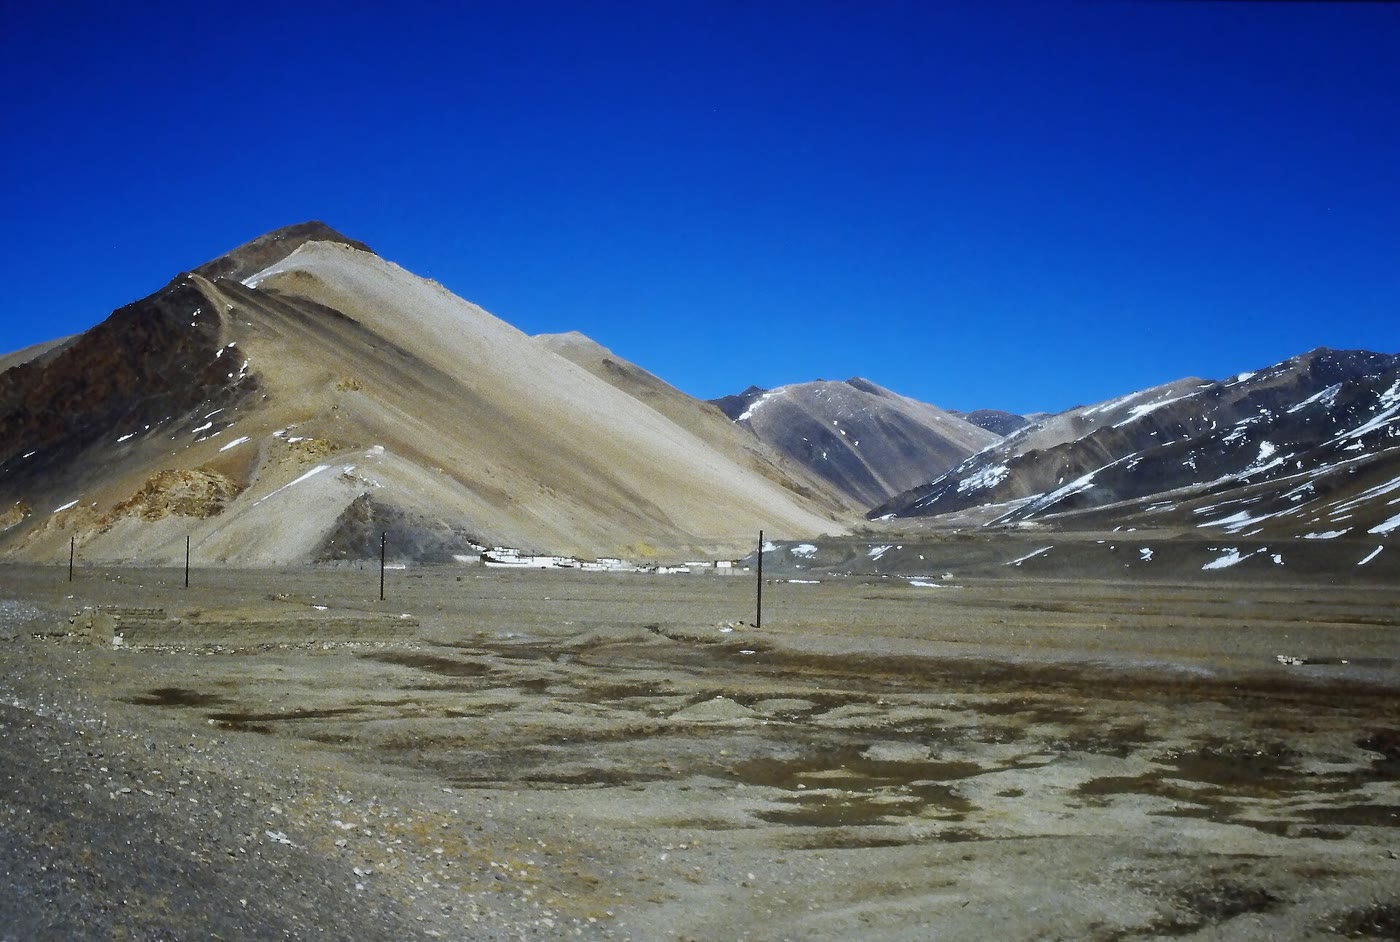
\includegraphics[width=0.66\linewidth]{images/book4/b2-14-tibet-plateau.jpg}
\par\smallskip{\small 尼泊尔与日喀则之间的西藏高原：平坦的砾石与稀疏牧场构成的地面，
其间有一座村庄，夹在覆盖岩屑堆的裸露山地之间，
整体高出海平面四千米以上。
照片：Jan Kranendonk，1987，CC BY-SA 4.0。}
\end{omfigure}
% ledger: data:b4-etopo-tibet

\subsection{高原的重量}

高原对其周围施加着重量。在直到其根部底面的每一深度处，高原之下的
柱体所受的压强都比紧邻低地之下的柱体更高；
只有在补偿深度处，二者才相等。高柱体向外推挤。

\begin{proposition}[高原的额外势能]\label{prop:b2:himalaya-andes:gpe}
在\cref{prop:b2:himalaya-andes:airy}的假设下，取重力加速度为 $g$，对
高原柱体相对正常柱体的额外静岩压力，从高原顶面
积分至根部底面处的补偿深度（根的厚度为 $r$），其值为
\[
  \Delta F = \rho_c g h \left(H + \frac{h}{2} + \frac{r}{2}\right) .
\]
它是高原柱体单位面积的额外重力势能，也是高原
边缘单位长度上施加于
周围地区的推力。
\end{proposition}

\begin{proof}
自海平面起向下度量深度 $z$。在高原柱体中，压强为 $p_1 =
\rho_c g (z + h)$，自 $z = -h$ 到 $L = H + r$。在正常柱体中，海平面以上压强为零，
地壳中为 $\rho_c g z$，其下为 $\rho_c g H + \rho_m g (z - H)$。压差 $p_1
- p_0$ 自 $z = -h$ 处的 0 升至海平面处的 $\rho_c g h$，并在正常地壳中保持该值，
此处两柱体均为地壳；在 $z = H$ 以下，压差线性减小，减小率为每米
$(\rho_m - \rho_c) g$，并在 $L$ 处降为零，因为 $(\rho_m - \rho_c) r = \rho_c
h$。积分即为该梯形的面积：$\rho_c g h\,(h/2 + H + r/2)$。两柱体侧向交换物质时，
压力所做的功恰为此积分，这正是它
既度量能量，也度量推力的原因。
\end{proof}

\begin{omfigure}
\centering
% figdata/bachelor-2/plateaus.py part pressure (h = 4.8 km, H = 35 km, 2700 and 3300 kg/m3)
\begin{tikzpicture}
\begin{axis}[width=0.62\linewidth, height=5.6cm, y dir=reverse, xmin=0, xmax=160, ymin=-12,
  ymax=60, xlabel={额外压强 $p_1 - p_0$（\unit{MPa}）}, ylabel={海平面以下深度
  （\unit{km}）}, tick label style={font=\scriptsize}, label style={font=\small},
  xtick pos=bottom, ytick pos=left, clip=false]
\addplot[fill=omThm!20, draw=omThm, line width=1pt] table[x expr=\thisrow{p_high_MPa}-\thisrow{p_ref_MPa}, y=z_km] {figdata/out/bachelor-2-plateaus-pressure.dat} \closedcycle;
\draw[dashed] (axis cs:0,0) -- (axis cs:160,0);
\draw[dashed] (axis cs:0,35) -- (axis cs:160,35);
\draw[dashed] (axis cs:0,56.6) -- (axis cs:160,56.6);
\node[font=\scriptsize, anchor=north east] at (axis cs:160,0) {海平面};
\node[font=\scriptsize, anchor=north east] at (axis cs:160,35) {正常莫霍面，$H$};
\node[font=\scriptsize, anchor=south east] at (axis cs:160,56.6) {根部底面，$H + r$};
\node[font=\scriptsize, anchor=west] at (axis cs:100,-8.4) {高原顶面，$-h$};
\node[font=\scriptsize, align=center] at (axis cs:60,20) {面积 $= \Delta F$\\$\approx\qty{6.1e12}{N.m^{-1}}$};
\end{axis}
\end{tikzpicture}
\par\smallskip{\small 高原柱体相对于正常
柱体的额外静岩压力；对于 $h = \qty{4.8}{km}$、$H = \qty{35}{km}$，密度分别为 2700 与
\qty{3300}{kg.m^{-3}}：它在高原内升高，在正常地壳中保持为 $\rho_c g h = \qty{127}{MPa}$，
并在根部底面降至零。阴影面积即为
\cref{prop:b2:himalaya-andes:gpe}所定义的额外势能。}
\end{omfigure}
% values (plateaus.py): tibet_gpe 6.12179e12 N/m for h = 4.8

对西藏而言，$r = 4.5 \times 4.8 = \qty{21.6}{km}$，而 $\Delta F = 2700 \times 9.8 \times 4800
\times (35000 + 2400 + 10800) \approx \qty{6.1e12}{N.m^{-1}}$。若将其分布于
厚度为 \qty{100}{km} 的岩石圈上，相当于约 \qty{60}{MPa} 的平均额外应力，与
使岩石破裂的应力同一量级。如此厚重的高原不能再简单地隆起，它倾向于向外扩展。

\begin{definition}[重力垮塌]\label{def:b2:himalaya-andes:collapse}
\omterm{def:b2:alpine-orogen:orogen}{造山带}的\emph{重力垮塌}\index{重力垮塌（造山带）}
是指增厚地壳在自身重量下的扩展，通过高地区的伸展，
以及边缘的向外流动或逆冲实现，其动力来自
增厚柱体的额外势能。
\end{definition}

西藏正被拉伸，而印度仍在推挤它。横跨藏南，南北向
裂谷切割高原并容纳东西向伸展，合计约 $9 \pm \qty{2}{mm}$ 每年，
位于 \ang{81} 至 东经 \ang{92} 之间；仅亚东–古鲁裂谷一处即约为 $1.3 \pm \qty{0.3}{mm}$ 每年，
尼泊尔以北的 GPS 测站显示，南部高原正在伸展，每年约
\num{12e-9}。地震记录也指向同一结论：逆冲断层与\omterm{def:b2:himalaya-andes:thickening}{地壳增厚}
主导高原周围的低地，走滑断层与正断层则主要位于其内部。
其伸展的成因仍有争议。在东部高原，伸展被解读为
由高原自重驱动的\omterm{def:b2:himalaya-andes:collapse}{重力垮塌}；在南部，另有学者将其与喜马拉雅弧的弯曲形状联系起来，
沿此弧的逆冲带呈发散状，或归因于印度向其下方滑入。
% ledger: wang21:rifts, ader12:extension

\subsection{侧向逃逸}

\begin{definition}[侧向挤出]\label{def:b2:himalaya-andes:extrusion}
\emph{侧向挤出}\index{侧向挤出}（逃逸构造）是指地壳或岩石圈块体
从碰撞带沿大型走滑断层向侧方挤出，
其方向大致垂直于汇聚方向，朝向一个自由边界。
\end{definition}

西藏以东，亚洲并非只是缩短，还被推向一侧。长距离的左行走滑断层，
其中包括红河断裂与阿尔金断裂，被认为引导了
大型块体向东及东南方向的逃逸，先是东南亚的巽他地块，
随后是西藏与华南，同时其远端张开了裂谷与年轻的洋盆。
在将刚性压模压入橡皮泥层的实验中，产生了此类断层；
而将亚洲视为连续黏性薄板的模型，则产生大范围的增厚，
且没有大断层。GPS 数据支持块体运动：相对于稳定的西伯利亚，塔里木
盆地大致向北运动，速率约 \qty{14}{mm} 每年，华南则向东南偏东
运动，速率约 \qty{8}{mm} 每年。印度推进的量中，有多少由增厚吸收，有多少
由挤出吸收，目前仍有争议。
% ledger: jiao23:extrusion

\section{安第斯山脉}\label{sec:b2:himalaya-andes:andes}

纳斯卡板块以约 \qty{72}{mm} 每年的速率俯冲到南美洲之下，位于
南纬 \ang{20} 附近，朝东北偏东方向运动（依 NNR-MORVEL56 角速度）。此处并无
大陆块体抵达，然而中安第斯山却承载着地球上第二高的高原。
% ledger: nnr56:poles
% values (plateaus.py): v_nazca_southamerica 72.52 mm/yr, azimuth 74.5

自西向东，在约 \ang{15} 至 南纬 \ang{27} 之间，它们包括五个带：
\emph{弧前}；\emph{西科迪勒拉}，即火山弧；高原，北段为
\emph{阿尔蒂普拉诺}，南段为\emph{普纳}；\emph{东科迪勒拉}；
以及薄皮\omterm{def:b2:alpine-orogen:ftb}{褶皱–冲断带}的\emph{次安第斯带}，它过渡为
查科平原。上图在 南纬 \ang{20} 处穿过这些单元：自海沟起，
其最深节点位于 西经 \ang{71.4} 处、海平面以下 \qty{7.7}{km}，地表
抬升超过 \qty{11}{km}，在约 \qty{240}{km} 的距离内到达 西经 \ang{69.1} 处的高原边缘；
高原在 \qty{440}{km} 的范围内保持在 \qty{3000}{m} 以上，平均
海拔为 \qty{3760}{m}。阿尔蒂普拉诺的平均高度为 \qty{3.7}{km}，普纳的平均高度为
\qty{4.4}{km}。在 南纬 \ang{23} 以北，莫霍面通常深于 \qty{60}{km}；在
中部阿尔蒂普拉诺之下，地壳厚 59 至 \qty{64}{km}。
% ledger: gerbault05:andes, gerbault05:moho, data:b4-etopo-andes

\begin{omfigure}
\centering
\begin{tikzpicture}[x=0.56cm, y=0.38cm, font=\scriptsize]
% mantle background
\fill[gray!12] (0,-2.6) -- (5,-3.6) -- (8,-5.6) -- (10,-9.1) -- (12,-12.6) -- (13.2,-14.6) -- (26,-14.6)
  -- (26,-4.5) -- (20,-4.7) -- (17.5,-6.0) -- (15,-7.3) -- (11,-7.0) -- (9.5,-6.2) -- (8,-4) -- (5,-2)
  -- (0,-1) -- cycle;
% ocean water
\fill[blue!8] (0,0) -- (6.33,0) -- (5,-2) -- (0,-1) -- cycle;
% Nazca slab
\fill[gray!45] (0,-1) -- (5,-2) -- (8,-4) -- (10,-7.5) -- (12,-11) -- (14,-14.5) -- (13.2,-14.6)
  -- (12,-12.6) -- (10,-9.1) -- (8,-5.6) -- (5,-3.6) -- (0,-2.6) -- cycle;
% South American crust
\fill[orange!22] (5,-2) -- (8,1) -- (9,1.9) -- (10.2,2.0) -- (11,2.0) -- (15,2.0) -- (15.6,2.6) -- (16.8,2.4)
  -- (17.5,1.6) -- (20,0.6) -- (20.6,0.4) -- (26,0.3) -- (26,-4.5) -- (20,-4.7) -- (17.5,-6.0) -- (15,-7.3)
  -- (11,-7.0) -- (9.5,-6.2) -- (8,-4) -- cycle;
% Altiplano basin fill
\fill[yellow!45] (11,2.0) -- (15,2.0) -- (14.6,1.0) -- (11.4,1.0) -- cycle;
% surface line
\draw[line width=0.5pt] (0,-1) -- (5,-2) -- (8,1) -- (9,1.9) -- (10.2,2.0) -- (11,2.0) -- (15,2.0) -- (15.6,2.6)
  -- (16.8,2.4) -- (17.5,1.6) -- (20,0.6) -- (20.6,0.4) -- (26,0.3);
% arc volcanoes
\fill[red!60!black] (8.8,1.75) -- (9.2,2.9) -- (9.6,1.95) -- cycle;
\fill[red!60!black] (9.8,1.95) -- (10.2,2.8) -- (10.6,2.0) -- cycle;
\draw[red!60!black, decorate, decoration={snake, amplitude=0.6pt, segment length=4pt}] (10.8,-8.0) -- (9.9,1.6);
% Subandean decollement and splays
\draw[thick] (16.0,-1.2) -- (20.55,0.42);
\draw (17.4,-0.7) -- (17.85,1.45);
\draw (18.4,-0.35) -- (18.8,1.08);
\draw (19.4,0.0) -- (19.7,0.72);
% Moho
\draw[dashed] (8,-4) -- (9.5,-6.2) -- (11,-7.0) -- (15,-7.3) -- (17.5,-6.0) -- (20,-4.7) -- (26,-4.5);
% labels
\node at (2.6,-0.5) {太平洋};
\node at (2.4,-2.2) {纳斯卡板块};
\draw[-{Latex[length=1.6mm]}] (1.6,-2.8) -- (3.2,-3.0);
\node[anchor=south] (tr) at (4.3,0.9) {海沟};
\draw[->] (tr.south) -- (5,-1.8);
\node[anchor=south east] at (7.6,1.0) {弧前};
\node[anchor=south, align=center] at (9.7,3.0) {西科迪勒拉 \\（火山弧）};
\node[anchor=south] at (13,2.1) {阿尔蒂普拉诺};
\node[anchor=south, align=center] at (16.4,2.7) {东科迪勒拉};
\node[anchor=south west] at (18.6,1.3) {次安第斯};
\node[anchor=south] at (23.5,0.4) {查科平原};
\node at (13,-3.2) {厚地壳};
\node at (23.2,-2.0) {巴西地盾};
\node[anchor=north] at (23.2,-4.6) {莫霍面};
\node at (14.2,-9.6) {地幔楔};
\node at (21,-10) {地幔};
\node[rotate=-50] at (12.75,-12.9) {板片};
\draw[-{Latex[length=2mm]}] (1.2,4.6) -- (0.2,4.6);
\node[anchor=south] at (0.7,4.6) {西};
\draw[-{Latex[length=2mm]}] (24.8,4.6) -- (25.8,4.6);
\node[anchor=south] at (25.3,4.6) {东};
\end{tikzpicture}
\par\smallskip{\small 沿 南纬 \ang{20} 附近穿过中部安第斯山脉的示意剖面（不
按比例）。纳斯卡板块俯冲于弧前之下，\omterm{def:b2:magma-emplacement:magma}{岩浆}自地幔楔（波浪线）上升
至西科迪勒拉的火山弧；阿尔蒂普拉诺以其厚的盆地充填物，位于
两条科迪勒拉之间，位于厚约 \qty{60}{km} 的地壳之上；薄皮
次安第斯带向东逆冲于巴西地盾之上。}
\end{omfigure}
% ledger: gerbault05:andes, gerbault05:moho

\subsection{地壳是如何增厚的}

阿尔蒂普拉诺额外的地壳从何而来？第一种可能是缩短作用：
挤压一条地壳带，它会增厚，而其截面积保持不变。

\begin{proposition}[缩短导致的增厚]\label{prop:b2:himalaya-andes:shortening}
设厚度均匀为 $H$ 的地壳在不增不减岩石的条件下被缩短，
变为厚度为 $T$、宽度为 $W$ 的地壳，剖面保持与缩短方向平行。其
原始宽度为 $W_0 = W T/H$，缩短量为
\[
  S = W_0 - W = W\,\frac{T - H}{H} .
\]
\end{proposition}

\begin{proof}
地壳的截面积守恒，与
\cref{prop:b2:alpine-orogen:balance}中的面积平衡一致：$W_0 H = W T$。因此 $W_0 = WT/H$，$S = W_0 - W =
W(T - H)/H$。
\end{proof}

在 南纬 \ang{20} 处，高原宽约 \qty{440}{km}；若其地壳厚约 \qty{60}{km}，
原先约为 \qty{35}{km}，则所需缩短量为 $440 \times 25/35 \approx \qty{314}{km}$。
在 16--南纬 \ang{21} 附近的\omterm{def:b2:alpine-orogen:balanced}{平衡剖面}显示，阿尔蒂普拉诺的缩短量约为 \qty{50}{km}，
次安第斯带自渐新世以来的缩短量超过 \qty{200}{km}。由缩短量算得的地壳体积
比由莫霍面深度算得的少约 \qty{20}{\percent}，
这一差异部分可能源于错误的假设，涉及初始厚度或地震莫霍面的性质；
另一部分可能是以其他方式增加的地壳。一项在
南纬 \ang{21} 附近的汇编研究认为，构造缩短至少占地壳根部的 \qty{55}{\percent}，
弧前地幔楔的水合作用至多占 \qty{20}{\percent}，\omterm{def:b2:magma-emplacement:magma}{岩浆}添加与
构造侵蚀仅约占 \qty{5}{\percent}。\omterm{def:b2:alpine-orogen:orogen}{造山带}内部的岩石也可能移动：
地壳厚度的差异会产生势能差，如西藏的情形，
这种势能差可驱动炽热的下地壳由厚处流向薄处。
% ledger: gerbault05:andes, gerbault05:volume, gerbault05:moho, data:b4-etopo-andes

\begin{omfigure}
\centering
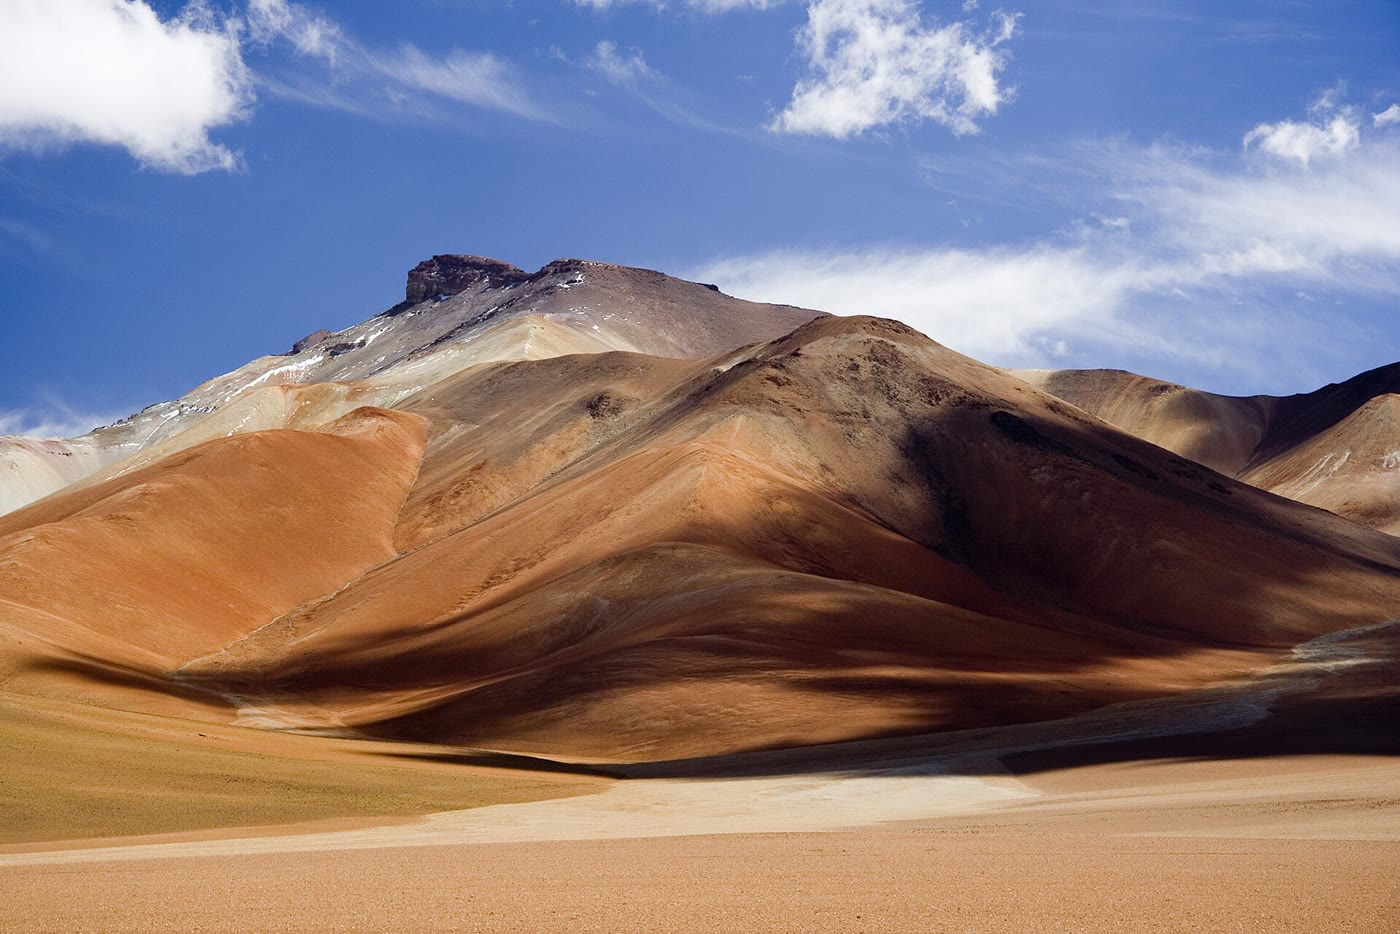
\includegraphics[width=0.66\linewidth]{images/book4/b2-14-altiplano.jpg}
\par\smallskip{\small 玻利维亚阿尔蒂普拉诺：山脚下是砾石与沙构成的平原，
周围是裸露的丘陵，因岩石而呈红色、赭色和灰色。照片：Luca Galuzzi, 2006, CC BY-SA 2.5。}
\end{omfigure}
% ledger: gerbault05:andes

\subsection{平板俯冲与失落的根}

板片的倾角并不固定，而这对地表有重要影响。

\begin{definition}[平板俯冲]\label{def:b2:himalaya-andes:flat-slab}
\emph{平板俯冲}\index{平板俯冲}是指板片在首次下倾之后，
几乎水平地在上覆板块之下延伸，
数百千米，然后再次下沉。
\end{definition}

今天，安第斯山脉下的纳斯卡板片有两段呈平板状：秘鲁段
自约 \qty{15}{Ma} 起呈平板状，潘帕段则自约 \qty{18}{Ma} 起如此。其上
没有活火山。潘帕板片变平之后，火山弧向内陆迁移，喷出的
熔岩减少；在平坦段之上，火山弧已经沉寂。本科一年级分册中的弧沟间隙
可以解释这种内移：火山弧下的板片越平缓，
板片抵达地幔楔熔融深度时离海沟就越远；若板片在该深度以上保持平坦，
就根本没有可以熔融的热地幔楔。
% ledger: gauthier24:flat

\begin{definition}[岩石圈拆沉]\label{def:b2:himalaya-andes:delamination}
\emph{岩石圈拆沉}\index{岩石圈拆沉}是指增厚岩石圈下部的脱离
并沉入软流圈之中，包括其地幔岩石圈，有时还包括致密的下地壳，
被热的软流圈取代。
\end{definition}

有人提出，南普纳之下存在拆沉作用，位于 \ang{24} 至 南纬 \ang{27} 之间，
时间约在 2 至 \qty{3}{Ma} 之前，那里喷出了年轻的镁铁质熔岩；沿高原一带，
地壳厚度与高程的变化，被认为与地幔岩石圈的去除有关，
南阿尔蒂普拉诺之下的地幔岩石圈已去除，中阿尔蒂普拉诺之下尚未完全去除。失去
致密的地幔盖层后，剩余岩柱变轻，地表无需再缩短即可抬升。
普纳高原比阿尔蒂普拉诺高约 \qty{1}{km}，地壳却薄约
\qty{11}{km}，这一反差要求普纳地壳较轻，
或其下地幔较轻。
% ledger: gerbault05:delamination, gerbault05:moho

\section{两个造山带的比较}\label{sec:b2:himalaya-andes:compared}

两个高原远看相似，而在其他几乎所有方面都不同，下表
将其归纳如下。

\begin{omfigure}
\centering\small
\begin{tabular}{>{\raggedright\arraybackslash}p{0.2\linewidth}|>{\raggedright\arraybackslash}p{0.34\linewidth}|>{\raggedright\arraybackslash}p{0.34\linewidth}}
 & 喜马拉雅与西藏 & 中部安第斯 \\ \hline
驱动机制 & 海洋闭合后陆块与陆块相撞 & 大洋板块俯冲到大陆之下 \\
轴线 & 带\omterm{def:b2:alpine-orogen:ophiolite}{蛇绿岩}的缝合带 & 板片之上的火山弧 \\
\omterm{def:b2:magma-emplacement:magma}{岩浆}活动 & 地壳熔融：\omterm{def:b2:crustal-melting:leucogranite}{淡色花岗岩} & 火山弧安山岩；岩石圈丢失处为镁铁质熔岩 \\
汇聚 & 每年约 \qty{45}{mm}，其中一半在山脉内被吸收 & 每年约 \qty{72}{mm}，大部分被俯冲消耗 \\
大地震 & 位于主冲断层（MHT），阿萨姆 1950，$M_w \approx 8.5$ & 位于俯冲界面，智利 1960，$M_w$ 9.5 \\
高原 & 平均 \qty{4.8}{km}，延伸 \qty{1180}{km}；地壳 70--\qty{75}{km} & 平均 \qty{3.8}{km}，延伸 \qty{440}{km}；地壳约 \qty{60}{km} \\
高原构造 & 东西向伸展、挤出 & 两翼缩短；有人提出拆沉 \\
前陆 & 印度–恒河前陆坳陷与西瓦利克\omterm{def:b2:alpine-orogen:foreland}{磨拉石} & 亚安第斯带与查科平原 \\
\end{tabular}
\par\smallskip{\small 两个\omterm{def:b2:alpine-orogen:orogen}{造山带}并列对比；文献来源见前文各节，
智利地震是 1900 年以来记录到的最大地震。}
\end{omfigure}
% ledger: lave00:setting, lave00:siwaliks, weinberg16:himalaya, ader12:mht, ader12:quakes, usgs:largest, gerbault05:andes, gerbault05:moho, gerbault05:delamination, nnr56:poles, data:b4-etopo-tibet, data:b4-etopo-andes, cattin01:crust, wang21:rifts, jiao23:extrusion

最深刻的差别在于下沉的是什么。在安第斯，大洋板块持续下沉，
绝大部分汇聚量，即每年约 \qty{72}{mm}，在海沟处被消耗；
若要在约 3000 万年内将上盘缩短 \qty{310}{km}，只需占其中每年约 \qty{10}{mm}。
在喜马拉雅，轻质物质无法长久下沉，因此汇聚量
全部用于叠置、增厚，并把亚洲推向一旁。两个\omterm{def:b2:alpine-orogen:orogen}{造山带}都能形成高原，因为\omterm{def:b2:himalaya-andes:thickening}{地壳增厚}即意味着地势增高；
两个高原都会在自身重量与边缘推力相平衡时停止抬升，
随后向外扩展。
% ledger: nnr56:poles, gerbault05:andes, ader12:mht, jiao23:extrusion

\section{山能有多高？}\label{sec:b2:himalaya-andes:heights}

最高峰珠穆朗玛峰，海拔 \qty{8848.86}{m}，依据的是
2020 年公布的联合测量结果。为何不能达到二十千米？一个粗略的界限来自岩石的强度。

\begin{proposition}[岩石强度给出的高度限制]\label{prop:b2:himalaya-andes:height}
一根密度为 $\rho$ 的岩柱，高出周围 $h$，其上方在周围水平面以上无侧向支撑，
底部承受竖直应力 $\rho g h$，并
在自由侧面上水平应力为零，因而差应力为 $\rho g h$。若岩石在差应力 $\sigma_d$ 下
发生破坏，则岩柱仅当 $h < \sigma_d/(\rho
g)$ 时方能保持稳定。
\end{proposition}

\begin{proof}
岩柱底部的竖直应力，即其上方岩石单位面积的重量，
$\rho g h$。侧面自由，因此该处水平应力为零。差应力
为最大与最小主应力之差，此处即 $\rho g h - 0$。
只有保持在 $\sigma_d$ 以下，才能避免破坏。
\end{proof}

实际山体有倾斜的侧翼约束其核心，因此其下的应力
较小；作数量级估计，取其一半，即 $\rho g h/2$。对珠穆朗玛峰，$2700 \times 9.8
\times 8849/2 \approx \qty{117}{MPa}$。本科一年级分册中的拜尔利定律给出，断层上岩石的摩擦强度，
在正应力 \qty{200}{MPa} 下为 $50 + 0.6 \times 200 =
\qty{170}{MPa}$，两者量级相同。若山体高出三倍，其底部所受荷载将远超岩石所能承受的范围，
山体会破坏并向外扩展。地球上八至九千米的山峰
已接近极限，而高原在山峰破坏之前早已扩展，
其海拔在五千米左右趋于稳定。
% ledger: tht:everest, byerlee:1975

\section*{练习}\label{sec:b2:himalaya-andes:exercises}

练习数据：$g = \qty{9.8}{m.s^{-2}}$；地壳与地幔密度
分别为 \qty{2700}{kg.m^{-3}} 与 \qty{3300}{kg.m^{-3}}，除非另有说明；正常地壳 $H =
\qty{35}{km}$。

\begin{exercise}[$\star$]\label{exo:b2:himalaya-andes:1}
某高原平均海拔为 \qty{3.0}{km}。利用
\cref{prop:b2:himalaya-andes:airy}，求 (a) 其艾里根；(b) 其地壳厚度。
(c) 若地壳再增加 \qty{10}{km}，它将升高多少？
\end{exercise}

\begin{exercise}[$\star$]\label{exo:b2:himalaya-andes:2}
一条穿越尼泊尔喜马拉雅的剖面，从恒河平原延伸至青藏高原。
(a) 按顺序列出其所穿越的地质单元及分隔它们的断层；(b) 哪条断层
是正断层？(c) 向北直至大喜马拉雅岩系，变质级如何变化，
以及其上方又如何变化？
\end{exercise}

\begin{exercise}[$\star$]\label{exo:b2:himalaya-andes:3}
尼泊尔中部一处于 \qty{9.2}{ka} 前废弃的河流阶地，
已跨越主前缘逆冲断层的褶皱缩短了 \qty{196.5}{m}。(a) 求平均缩短速率，
以毫米每年计；(b) 将其与跨越山脉的 GPS 汇聚量相比较，该汇聚量为
\qty{17.8}{mm} 每年。(c) 这一吻合对 MFT 以北的断层说明了什么？
\end{exercise}

\begin{exercise}[$\star$]\label{exo:b2:himalaya-andes:4}
将下列每项观察归入\omterm{def:b2:himalaya-andes:types}{碰撞造山带}、\omterm{def:b2:himalaya-andes:types}{安第斯型造山带}或两者兼有：(a) 一条衬有\omterm{def:b2:alpine-orogen:ophiolite}{蛇绿岩}的缝合带；
(b) 一列活动的安山质火山；(c) 由地壳熔融形成的\omterm{def:b2:crustal-melting:leucogranite}{淡色花岗岩}；
(d) 沿前缘分布的深海沟；(e) 含\omterm{def:b2:alpine-orogen:foreland}{磨拉石}的\omterm{def:b2:alpine-orogen:foreland}{前陆盆地}；
(f) 山脉之下平缓倾斜的断层上发生的大地震。
\end{exercise}

\begin{exercise}[$\star\star$]\label{exo:b2:himalaya-andes:5}
印度相对欧亚板块，以每年 \qty{45}{mm} 的速度穿越喜马拉雅山脉；在尼泊尔境内，
山脉本身东段每年吸收 \qty{17.8}{mm}，西段每年吸收 \qty{20.5}{mm}。
(a) 两种情况下，山脉各吸收了汇聚量的多大比例？(b) 其余部分
去了哪里？(c) 在 \qty{10}{Ma} 内，剩余部分代表多大的缩短量？
\end{exercise}

\begin{exercise}[$\star\star$]\label{exo:b2:himalaya-andes:6}
(a) 利用\cref{prop:b2:himalaya-andes:gpe}，求
阿尔蒂普拉诺高原（平均海拔 \qty{3.7}{km}）的超额重力势能。(b) 将其与海拔 \qty{4.8}{km} 的西藏相比较。
(c) 证明：对薄高原，$h \ll H$ 时 $\Delta F$ 与 $h$ 成正比，而对
厚高原则增长更快。这对高原的增长意味着什么？
\end{exercise}

\begin{exercise}[$\star\star$]\label{exo:b2:himalaya-andes:7}
(a) 求珠穆朗玛峰下方的 $\rho g h/2$，其高度为 \qty{8848.86}{m}，取 $\rho =
\qty{2700}{kg.m^{-3}}$。(b) 由拜尔利定律，$\tau = 0.85\,\sigma_n$ 用于正应力低于 \qty{200}{MPa} 的情形，
高于此值时 $\tau = \qty{50}{MPa} + 0.6\,\sigma_n$；求 $\tau$ 在 $\sigma_n =
100$ 和 \qty{200}{MPa} 下的值。(c) 若强度为 \qty{170}{MPa}，
按同一数量级规则，可允许的高度为多少？
\end{exercise}

\begin{exercise}[$\star\star$]\label{exo:b2:himalaya-andes:8}
藏南裂谷每年承担 $9 \pm \qty{2}{mm}$ 的东西向伸展，其范围位于
东经 \ang{81} 至 \ang{92} 之间。(a) 在北纬 \ang{30} 处，该段宽度为多少？已知子午线上每度 \qty{111.19}{km}。
(b) 计算平均伸展应变率，分别以每年和每秒计，
并给出其范围。(c) 将其与尼泊尔以北 GPS 测得的 $(12.4 \pm 4.7) \times 10^{-9}$ 每年相比较。
\end{exercise}

\begin{exercise}[$\star\star$]\label{exo:b2:himalaya-andes:9}
尼泊尔之下闭锁的主喜马拉雅逆冲断层每年积累的矩亏损为
\qty{6.6e19}{N.m}，而过去 500 年的地震每年仅释放
\qty{0.9e19}{N.m}。(a) 它们释放了亏损的多大比例？(b) 取 $M_0 =
10^{1.5 M_w + 9.1}$\,\unit{N.m}，求 $M_w$
为 8.5 的地震的力矩。(c) 此类地震需多久发生一次，才能平衡该亏损？
\end{exercise}

\begin{exercise}[$\star\star\star$]\label{exo:b2:himalaya-andes:10}
普纳高原比阿尔蒂普拉诺高原高 \qty{0.7}{km}（4.4 对 \qty{3.7}{km}），其下地壳
薄 \qty{11}{km}。取阿尔蒂普拉诺地壳厚 \qty{61.5}{km}，密度为
\qty{2800}{kg.m^{-3}}，两者之下的地幔密度均为 \qty{3300}{kg.m^{-3}}。(a) 写出
两柱在共同补偿深度以上质量相等的表达式。(b) 求
若仅地壳补偿该差异，普纳地壳必须具有的密度。(c) 与
所引的 150 至 \qty{200}{kg.m^{-3}} 相比较，并说明还有何因素可以解释这一反差。
\end{exercise}

\begin{exercise}[$\star\star\star$]\label{exo:b2:himalaya-andes:11}
火山前缘位于板片顶部深 \qty{105}{km} 处的正上方。(a) 对于板片，
均匀倾角为 \ang{30}，用本科一年级分册中的公式求弧沟间隙。
(b) 板片现在先以 \ang{30} 的倾角下倾至 \qty{90}{km} 深度，随后仅以 \ang{4} 倾斜：求
新的弧沟间隙及火山弧向陆地方向的位移量。(c) 若板片变平，
在 \qty{95}{km} 深度处保持 \qty{300}{km}，火山弧会如何变化？
\end{exercise}

\begin{exercise}[$\star\star\star$]\label{exo:b2:himalaya-andes:12}
侵蚀作用每百万年约移除喜马拉雅山脉每千米长度上的 \qty{300}{km^3} 岩石。
印度以每年 \qty{21}{mm} 的速度带入厚 \qty{37.5}{km} 的地壳。(a) 每千米山脉每百万年
有多少地壳进入\omterm{def:b2:alpine-orogen:orogen}{造山带}？(b) 其中被侵蚀移除的比例为多少？
(c) 其余部分可能在哪里？
\end{exercise}

\begin{problem}[{周末问题 --- 两个高原}]\label{pb:b2:himalaya-andes:1}
本章的条带剖面给出了横跨西藏
（\qtyrange{86}{90}{\degree} 东经）及横跨中安第斯山脉（\qtyrange{19}{21}{\degree} 南纬）的节点平均海拔。
以每 \ang{1.5} 纬度及每一度经度采样，并四舍五入至 \qty{10}{m}，
结果如下。除非另有说明，$g = \qty{9.8}{m.s^{-2}}$，$\rho_c = \qty{2700}{kg.m^{-3}}$，
$\rho_m = \qty{3300}{kg.m^{-3}}$，正常地壳厚度为 $H = \qty{35}{km}$。

\smallskip
\begin{center}\small
\begin{tabular}{l|ccccccccc}
纬度（\unit{\degree} 北） & 26.5 & 28.0 & 29.5 & 31.0 & 32.5 & 34.0 & 35.5 & 37.0 & 38.5 \\ \hline
平均海拔（\unit{m}） & 70 & 5000 & 5030 & 4830 & 5020 & 5150 & 5050 & 4470 & 2210
\end{tabular}

\smallskip
\begin{tabular}{l|cccccccc}
经度（\unit{\degree}） & $-71$ & $-70$ & $-69$ & $-68$ & $-67$ & $-66$ & $-65$ & $-64$ \\ \hline
平均海拔（\unit{m}） & $-3310$ & 970 & 4150 & 3720 & 3740 & 4010 & 3030 & 1170
\end{tabular}
\end{center}
\smallskip

\noindent\textbf{第一部分 --- 读取剖面。}
\begin{enumerate}
\item 取高于 \qty{3000}{m} 的样点作为高原，求西藏的
平均海拔 $h_T$，四舍五入至 \qty{0.1}{km}。
\item 对阿尔蒂普拉诺高原做同样计算，得到 $h_A$，并与所引的
阿尔蒂普拉诺平均高度 \qty{3.7}{km}、普纳高原 \qty{4.4}{km} 相比较。
\item 依据样点，每个高原至少有多宽（纬度每度 \qty{111.19}{km}；
经度每度在南纬 \ang{20} 处为 \qty{104.5}{km}）？
\item 求喜马拉雅前缘在北纬 \ang{26.5} 至 \ang{28.0} 之间的平均坡度，
以百分数表示。
\item 为什么安第斯剖面比西藏剖面不对称得多？
\end{enumerate}

\noindent\textbf{第二部分 --- 艾里厚度。}
\begin{enumerate}[resume]
\item 求西藏的艾里根及地壳厚度 $T_T$（由 $h_T$ 出发）。
\item 对阿尔蒂普拉诺高原做同样计算，求 $T_A$。
\item 将其与地震学厚度相比较：西藏之下为 70 至 \qty{75}{km}，
阿尔蒂普拉诺中部之下为 59 至 \qty{64}{km}。哪一个估计偏差更大？
\item 地壳密度为多少时，西藏的艾里厚度等于 \qty{72.5}{km}？
\item 密度取何值时，阿尔蒂普拉诺的厚度为 \qty{61.5}{km}？
\item 除地壳密度外，列举两个原因，说明局地艾里计算为何
可能遗漏观测到的根。
\item 印度之下地壳厚 \qty{37.5}{km}，西藏之下厚 \qty{72.5}{km}。取莫霍面处的密度差为
\qty{370}{kg.m^{-3}}，用布格板公式 $\Delta g
= 2\pi G\,\Delta\rho\,t$，估算西藏根相对印度的布格异常，$t$ 为
海平面以下的额外厚度（$G = \qty{6.674e-11}{m^3.kg^{-1}.s^{-2}}$）。将其与
观测到的 \qty{460}{mGal} 之差相比较。
\end{enumerate}

\noindent\textbf{第三部分 --- 缩短阿尔蒂普拉诺。}在 南纬 \ang{20}，高原
宽 \qty{440}{km}，地壳厚约 \qty{60}{km}。
\begin{enumerate}[resume]
\item 利用\cref{prop:b2:himalaya-andes:shortening}，计算恢复后的宽度，以及
若此前地壳厚 \qty{35}{km}，则所需的缩短量为多少。
\item \omterm{def:b2:alpine-orogen:balanced}{平衡剖面}给出阿尔蒂普拉诺约 \qty{50}{km} 的缩短量，以及
次安第斯带约 \qty{200}{km} 的缩短量。所需缩短量中有多大比例缺失？
\item 若缩短只使额外\omterm{def:b2:himalaya-andes:thickening}{地壳增厚} \qty{55}{\percent}，
则需要多大的缩短量？
\item 次安第斯带为\omterm{def:b2:alpine-orogen:skin}{薄皮构造}。其缩短为何仍须
在某处使\omterm{def:b2:himalaya-andes:thickening}{地壳增厚}？
\item 设第三部分的 \qty{314}{km} 是在 \qty{30}{Ma} 内积累的，计算平均
速率，以及它占今日纳斯卡板块–南美板块汇聚速率
（每年 \qty{72}{mm}）的比例。
\item 其余的汇聚去了何处？
\end{enumerate}

\noindent\textbf{第四部分 --- 西藏的重量。}
\begin{enumerate}[resume]
\item 利用\cref{prop:b2:himalaya-andes:gpe}，以 $h_T$ 计算西藏的
单位面积过剩势能。
\item 以 $h_A$ 计算阿尔蒂普拉诺的过剩势能，并求二者之比。
\item 将西藏的 $\Delta F$ 分摊到厚 \qty{100}{km} 的岩石圈上，
它代表多大的平均应力？
\item 藏南的伸展以每年 \qty{9}{mm} 的速率横跨 \qty{1060}{km}，
每年的应变为多少？
\item 印度仍在向北推挤，西藏为何能东西向伸展？
\item 总结：给出由平均海拔计算得到的西藏地壳厚度，
取整到千米，以及它占地震测得的 \qty{72.5}{km} 的比例。
\end{enumerate}
\end{problem}
